This report presents a length-based assessment of the status of the most abundant species of grouper caught in the multi-species deep demersal fisheries for snappers, groupers, and emperors in Eastern Indonesia. The gear types in these fisheries include vertical drop lines and bottom set long lines at various scales, ranging from small scale village based fisheries with boats less than 5 GT to medium scale drop line and long line vessels measuring up to well over 100 GT for the largest long line vessels. The drop line fishery is an active vertical hook and line fishery operating at depths from 50 to 500 meters, whereas long lines are set horizontally along the bottom at depths ranging from 50 to 150 meters.

The fisheries included in this report operate in Fisheries Management Areas (WPPs) 573, 712, 713, 714, 715 and 718 including the Northern Indian Ocean, Timor Sea, Java Sea, Makassar Strait, Bali Sea, Flores Sea, Banda Sea, Moluccas Sea, Timor Sea and Arafura Sea. Vessels operating in this region are originating from various ports throughout the country and may also operate in other WPPs at times. Data from 2014 through 2016 were accumulated for this assessment.

For a complete overview of the species composition of these drop line and long line fisheries please refer to the ID guide prepared for these fisheries:

\textbf{CLICK: }\href{http://72.14.187.103:8080/ifish/pub/TNC_FishID.pdf}{Link to on-line E-Book Species ID Guide}

For further background on species life history characteristics, and data-poor length based assessment methods, as applied in this report, please refer to the assessment guide that was separately prepared for these fisheries:

\textbf{CLICK: }\href{http://72.14.187.103:8080/ifish/pub/DeepSlopeSpeciesAssessmentTool.pdf}{Link to on-line E-Book Assessment Guide with Biological Information}

Since August 2015, all fish in the catch of cooperating vessels were photographed as they were caught. Fish were placed on top of measuring boards to enable sizing as well as identification from images. Photographs were taken by crew participating in our Crew Operated Data Recording System or CODRS. Images were analyzed by staff at our fisheries stations to generate species specific length frequency distributions that served as the input for length based assessments presented in this report.

Already since October 2014, fish landed at processing plants were measured there as part of a Smart Weighing and Measuring System (SWMS) intended to increase traceability and introduce species and size specific data collection in supply lines of target species. Data from our SWMS were used in the analysis up to October 2015, by which time they could be replaced with CODRS data on complete catches.

\begin{center}
\graphicspath{{/root/R-project/IFishGrouper/Images/}}
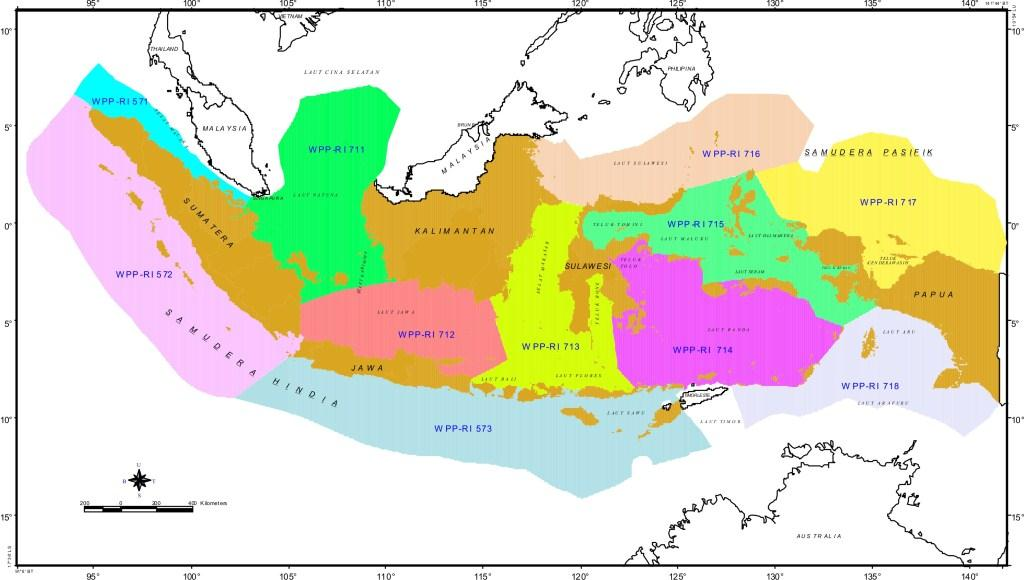
\includegraphics[scale=1.8]{wpp_indonesia.jpg}

Figure 1. Fisheries Management Areas (WPP) in Indonesian marine waters.
\end{center}

\begin{center}
\graphicspath{{/root/R-project/IFishGrouper/Images/}}
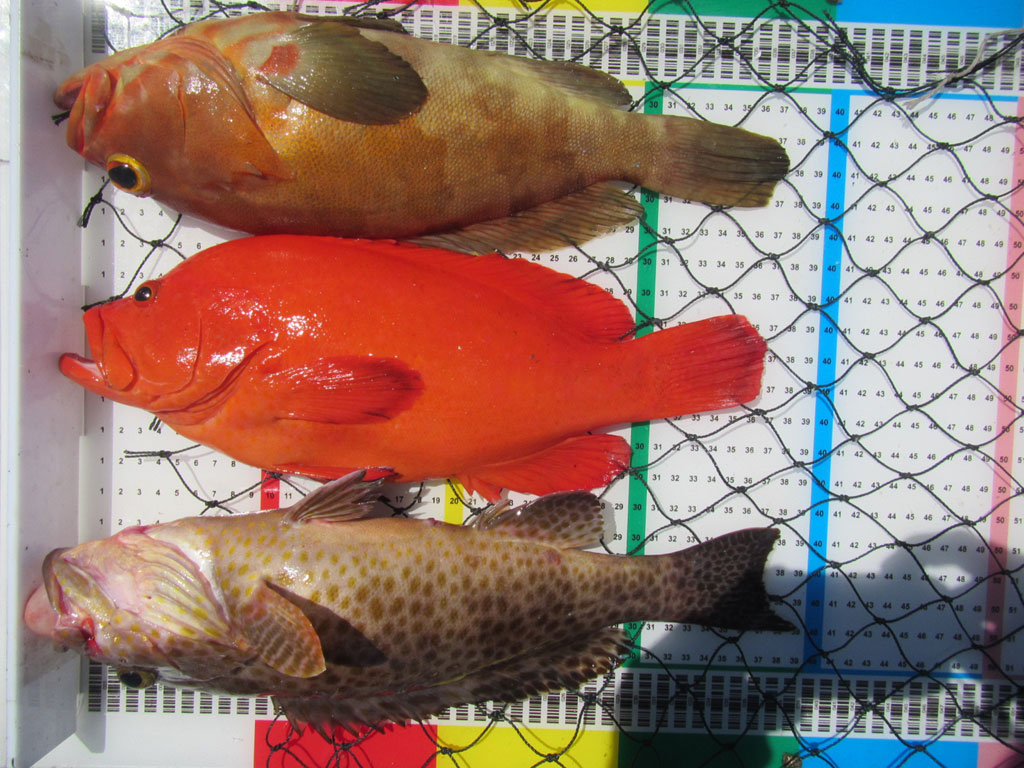
\includegraphics[scale=0.4]{codrs_grouper.jpg}

Figure 2. Groupers photographed by fishing crew on board as part of the Crew Operated Data Recording System (CODRS).
\end{center}